% Options for packages loaded elsewhere
% Options for packages loaded elsewhere
\PassOptionsToPackage{unicode}{hyperref}
\PassOptionsToPackage{hyphens}{url}
\PassOptionsToPackage{dvipsnames,svgnames,x11names}{xcolor}
%
\documentclass[
  letterpaper,
  DIV=11,
  numbers=noendperiod,
  openany]{scrreprt}
\usepackage{xcolor}
\usepackage{amsmath,amssymb}
\setcounter{secnumdepth}{5}
\usepackage{iftex}
\ifPDFTeX
  \usepackage[T1]{fontenc}
  \usepackage[utf8]{inputenc}
  \usepackage{textcomp} % provide euro and other symbols
\else % if luatex or xetex
  \usepackage{unicode-math} % this also loads fontspec
  \defaultfontfeatures{Scale=MatchLowercase}
  \defaultfontfeatures[\rmfamily]{Ligatures=TeX,Scale=1}
\fi
\usepackage{lmodern}
\ifPDFTeX\else
  % xetex/luatex font selection
\fi
% Use upquote if available, for straight quotes in verbatim environments
\IfFileExists{upquote.sty}{\usepackage{upquote}}{}
\IfFileExists{microtype.sty}{% use microtype if available
  \usepackage[]{microtype}
  \UseMicrotypeSet[protrusion]{basicmath} % disable protrusion for tt fonts
}{}
\makeatletter
\@ifundefined{KOMAClassName}{% if non-KOMA class
  \IfFileExists{parskip.sty}{%
    \usepackage{parskip}
  }{% else
    \setlength{\parindent}{0pt}
    \setlength{\parskip}{6pt plus 2pt minus 1pt}}
}{% if KOMA class
  \KOMAoptions{parskip=half}}
\makeatother
% Make \paragraph and \subparagraph free-standing
\makeatletter
\ifx\paragraph\undefined\else
  \let\oldparagraph\paragraph
  \renewcommand{\paragraph}{
    \@ifstar
      \xxxParagraphStar
      \xxxParagraphNoStar
  }
  \newcommand{\xxxParagraphStar}[1]{\oldparagraph*{#1}\mbox{}}
  \newcommand{\xxxParagraphNoStar}[1]{\oldparagraph{#1}\mbox{}}
\fi
\ifx\subparagraph\undefined\else
  \let\oldsubparagraph\subparagraph
  \renewcommand{\subparagraph}{
    \@ifstar
      \xxxSubParagraphStar
      \xxxSubParagraphNoStar
  }
  \newcommand{\xxxSubParagraphStar}[1]{\oldsubparagraph*{#1}\mbox{}}
  \newcommand{\xxxSubParagraphNoStar}[1]{\oldsubparagraph{#1}\mbox{}}
\fi
\makeatother


\usepackage{longtable,booktabs,array}
\usepackage{calc} % for calculating minipage widths
% Correct order of tables after \paragraph or \subparagraph
\usepackage{etoolbox}
\makeatletter
\patchcmd\longtable{\par}{\if@noskipsec\mbox{}\fi\par}{}{}
\makeatother
% Allow footnotes in longtable head/foot
\IfFileExists{footnotehyper.sty}{\usepackage{footnotehyper}}{\usepackage{footnote}}
\makesavenoteenv{longtable}
\usepackage{graphicx}
\makeatletter
\newsavebox\pandoc@box
\newcommand*\pandocbounded[1]{% scales image to fit in text height/width
  \sbox\pandoc@box{#1}%
  \Gscale@div\@tempa{\textheight}{\dimexpr\ht\pandoc@box+\dp\pandoc@box\relax}%
  \Gscale@div\@tempb{\linewidth}{\wd\pandoc@box}%
  \ifdim\@tempb\p@<\@tempa\p@\let\@tempa\@tempb\fi% select the smaller of both
  \ifdim\@tempa\p@<\p@\scalebox{\@tempa}{\usebox\pandoc@box}%
  \else\usebox{\pandoc@box}%
  \fi%
}
% Set default figure placement to htbp
\def\fps@figure{htbp}
\makeatother





\setlength{\emergencystretch}{3em} % prevent overfull lines

\providecommand{\tightlist}{%
  \setlength{\itemsep}{0pt}\setlength{\parskip}{0pt}}



 


\KOMAoption{captions}{tableheading}
\makeatletter
\@ifpackageloaded{bookmark}{}{\usepackage{bookmark}}
\makeatother
\makeatletter
\@ifpackageloaded{caption}{}{\usepackage{caption}}
\AtBeginDocument{%
\ifdefined\contentsname
  \renewcommand*\contentsname{Table of contents}
\else
  \newcommand\contentsname{Table of contents}
\fi
\ifdefined\listfigurename
  \renewcommand*\listfigurename{List of Figures}
\else
  \newcommand\listfigurename{List of Figures}
\fi
\ifdefined\listtablename
  \renewcommand*\listtablename{List of Tables}
\else
  \newcommand\listtablename{List of Tables}
\fi
\ifdefined\figurename
  \renewcommand*\figurename{Figure}
\else
  \newcommand\figurename{Figure}
\fi
\ifdefined\tablename
  \renewcommand*\tablename{Table}
\else
  \newcommand\tablename{Table}
\fi
}
\@ifpackageloaded{float}{}{\usepackage{float}}
\floatstyle{ruled}
\@ifundefined{c@chapter}{\newfloat{codelisting}{h}{lop}}{\newfloat{codelisting}{h}{lop}[chapter]}
\floatname{codelisting}{Listing}
\newcommand*\listoflistings{\listof{codelisting}{List of Listings}}
\makeatother
\makeatletter
\makeatother
\makeatletter
\@ifpackageloaded{caption}{}{\usepackage{caption}}
\@ifpackageloaded{subcaption}{}{\usepackage{subcaption}}
\makeatother
\usepackage{bookmark}
\IfFileExists{xurl.sty}{\usepackage{xurl}}{} % add URL line breaks if available
\urlstyle{same}
\hypersetup{
  pdftitle={Projeto Integrador I: Análise de Desempenho Acadêmico x Presença em Sala},
  pdfauthor={Ike Gabriel Rodrigues Kenard; Leonardo de Lima Amaral; Marcelo Saraiva Cavalvanti; Vitor Nascimento Franco; Rafael Mascarenhas Brown de Andrade; Alessandra de Souza Gonçalves; Rodrigo Lins Bezerra Magalhaes},
  colorlinks=true,
  linkcolor={blue},
  filecolor={Maroon},
  citecolor={Blue},
  urlcolor={Blue},
  pdfcreator={LaTeX via pandoc}}


\title{Projeto Integrador I: Análise de Desempenho Acadêmico x Presença
em Sala}
\author{Ike Gabriel Rodrigues Kenard \and Leonardo de Lima
Amaral \and Marcelo Saraiva Cavalvanti \and Vitor Nascimento
Franco \and Rafael Mascarenhas Brown de Andrade \and Alessandra de Souza
Gonçalves \and Rodrigo Lins Bezerra Magalhaes}
\date{2025-06-30}
\begin{document}
\maketitle

    % Contracapa
\begin{titlepage}
    \centering
    \vspace*{5cm}
    {\Large Universidade CEUB \par}
    \vspace{0.5cm}
    {\large Projeto Integrador I \par}
    \vspace{0.5cm}
    {\large Grupo Ike - Análise Rendimento Acadêmico\par}
    \vspace{1cm}
    {\large Brasília \par}
    {\large 2025 \par}
\end{titlepage}

\renewcommand*\contentsname{Table of contents}
{
\hypersetup{linkcolor=}
\setcounter{tocdepth}{2}
\tableofcontents
}

\bookmarksetup{startatroot}

\chapter{Apresentação Geral}\label{apresentauxe7uxe3o-geral}

Este relatório tem como objetivo apresentar o desenvolvimento do Projeto
Integrador I do curso de Ciência de Dados e Machine Learning do Centro
Universitário de Brasília (CEUB). O projeto foi idealizado com foco na
automatização da coleta de presença dos alunos em sala de aula e na
análise da relação entre frequência e desempenho acadêmico, utilizando
conceitos e ferramentas de ciência de dados.

A proposta surgiu da necessidade de tornar o processo de chamada mais
eficiente, confiável e capaz de fornecer informações relevantes para a
gestão acadêmica. Para isso, foi projetado um sistema que integra
hardware (RFID UHF), backend (API para ingestão de dados em tempo real),
pipelines de tratamento e dashboards analíticos.

Do ponto de vista analítico, o projeto aplica técnicas de Análise de
Séries Temporais para compreender como a frequência dos estudantes
evolui ao longo do tempo e de que forma ela se correlaciona com suas
notas. Essa abordagem visa oferecer insights acionáveis para professores
e coordenadores sobre o comportamento dos alunos.

O trabalho está estruturado em cinco capítulos, além desta introdução:

\begin{itemize}
\tightlist
\item
  \textbf{Capítulo 1 -- Introdução}: apresenta o problema, os objetivos
  e a justificativa da proposta.
\item
  \textbf{Capítulo 2 -- Metodologia}: descreve as etapas de
  desenvolvimento e as ferramentas utilizadas.
\item
  \textbf{Capítulo 3 -- Desenvolvimento}: detalha a implementação das
  tecnicas utilzadas e análises feitas.
\item
  \textbf{Capítulo 4 -- Resultados}: exibe gráficos, análises e métricas
  obtidas.
\item
  \textbf{Capítulo 5 -- Conclusão}: discute os aprendizados e as
  possibilidades de evolução do projeto.
\end{itemize}

Espera-se que esta iniciativa contribua para uma gestão educacional mais
inteligente, baseada em dados confiáveis e análises precisas.

\bookmarksetup{startatroot}

\chapter{Objetivos e Motivações:}\label{objetivos-e-motivauxe7uxf5es}

Historicamente, a presença dos estudantes em sala de aula está ligada a
um desempenho acadêmico superior. Este projeto visa examinar a conexão
entre a presença dos alunos e seus resultados finais, bem como provar
que a viabilidade do RFID para uma melhor auxílio acadêmico

Através da avaliação de registros históricos de presença e notas, nosso
objetivo é produzir percepções que fundamentem e fortifiquem a
implementação de um sistema automatizado de controle de frequência nas
instituições educacionais.

O primeiro passo emprega algoritmos de aprendizado de máquina, mais
especificamente um Random Forest Regressor (RFR) e uma Regressão Linear
(RL), para analisar o efeito da frequência no rendimento escolar. Esta
avaliação tem como objetivo fundamentar as decisões dos interessados e
apoiadores do projeto.

A importância desta pesquisa está na procura por soluções que aprimorem
os processos acadêmicos, aprimorem o monitoramento dos estudantes e,
consequentemente, auxiliem na melhoria da qualidade da educação.

\section{Relatório de Entregas da
Equipe}\label{relatuxf3rio-de-entregas-da-equipe}

Este relatório detalha as principais contribuições de cada membro da
equipe nas entregas do projeto:

\begin{itemize}
\tightlist
\item
  Alessandra Gonçalves: Realizou a correção e revisão final dos textos.
\item
  Ike Kenard: Responsável pela organização de 90\% da documentação,
  incluindo a reestruturação de gráficos e a revisão de textos do
  documento principal.
\item
  Leonardo Amaral: Desenvolveu as duas apresentações do projeto e a
  estrutura geral do mesmo.
\item
  Marcelo Cavalcanti: Realizou a análise estatística e desenvolveu o
  modelo do projeto.
\item
  Rafael Andrade: Conduziu a análise de dados de Business Intelligence
  (BI).
\item
  Rodrigo Magalhaes: Conduziu a pesquisa de bases de dados relevantes.
\item
  Vitor Franco: Elaborou os textos e gerou os gráficos presentes no
  documento.
\end{itemize}

\bookmarksetup{startatroot}

\chapter{Métodologia:}\label{muxe9todologia}

Este projeto fez uso de informações públicas sobre o rendimento de
alunos do ensino secundário de duas instituições de ensino portuguesas:
Gabriel Pereira (GP) e Mousinho da Silveira (MS). A coleta de dados
ocorreu através de relatórios escolares e questionários aplicados aos
estudantes.

O dataset possui características associadas a:

\begin{itemize}
\tightlist
\item
  Notas dos três períodos (G1, G2, G3).
\item
  Informações demográficas: idade, gênero, local de residência (urbano
  ou rural), número de membros da família e outros.
\item
  Fatores sociais: situação familiar, conexão com a internet, conexão
  amorosa, entre outros.
\item
  Elementos acadêmicos: horas de estudo por semana, atividades
  extracurriculares, suporte educacional, ausências e reprovações
  passadas.
\end{itemize}

\section{Dicionário de Variáveis}\label{dicionuxe1rio-de-variuxe1veis}

\begin{itemize}
\tightlist
\item
  \textbf{school:} escola do estudante (GP ou MS)
\item
  \textbf{sex:} gênero (F ou M)
\item
  \textbf{age:} idade (15 a 22 anos)
\item
  \textbf{address:} tipo de endereço (U - urbano, R - rural)
\item
  \textbf{famsize:} tamanho da família (LE3 ≤ 3, GT3 \textgreater{} 3)
\item
  \textbf{Pstatus:} situação de coabitação dos pais (T - juntos, A -
  separados)
\item
  \textbf{reason:} motivo para escolha da escola (home, reputation,
  course, other)
\item
  \textbf{Mjob / Fjob:} profissão da mãe/pai (teacher, health, services,
  at\_home, other)
\item
  \textbf{Medu / Fedu:} escolaridade da mãe e do pai (0 a 4)
\end{itemize}

\begin{longtable}[]{@{}cl@{}}
\toprule\noalign{}
Código & Nível de Educação dos responsáveis \\
\midrule\noalign{}
\endhead
\bottomrule\noalign{}
\endlastfoot
\textbf{0} & nenhum \\
\textbf{1} & Fundamenal I \\
\textbf{2} & Fundamenal II \\
\textbf{3} & Ensino Médio \\
\textbf{4} & Ensin Superior \\
\end{longtable}

\begin{itemize}
\tightlist
\item
  \textbf{guardian:} responsável (mother, father, other)
\item
  \textbf{traveltime:} tempo de deslocamento até a escola (1 -
  \textless15min a 4 - \textgreater1h)
\item
  \textbf{studytime:} tempo de estudo semanal (1 - \textless2h a 4 -
  \textgreater10h)
\item
  \textbf{failures:} número de reprovações anteriores (0 a 4)
\item
  \textbf{schoolsup:} apoio educacional extra (yes/no)
\item
  \textbf{famsup:} apoio da família (yes/no)
\item
  \textbf{paid:} aulas extras pagas (yes/no)
\item
  \textbf{activities:} atividades extracurriculares (yes/no)
\item
  \textbf{nursery:} frequentou pré-escola (yes/no)
\item
  \textbf{higher:} desejo de cursar ensino superior (yes/no)
\item
  \textbf{internet:} acesso à internet em casa (yes/no)
\item
  \textbf{romantic:} possui relacionamento amoroso (yes/no)
\item
  \textbf{famrel:} qualidade do relacionamento familiar (1 - ruim a 5 -
  excelente)
\item
  \textbf{freetime:} tempo livre após a escola (1 a 5)
\item
  \textbf{goout:} frequência de saída com amigos (1 a 5)
\item
  \textbf{Dalc:} consumo de álcool durante a semana (1 a 5)
\item
  \textbf{Walc:} consumo de álcool no final de semana (1 a 5)
\item
  \textbf{health:} estado de saúde (1 - muito ruim a 5 - muito bom)
\item
  \textbf{absences:} número de faltas (0 a 93)
\end{itemize}

\section{Variáveis de Notas:}\label{variuxe1veis-de-notas}

G1: nota do 1º período (0 a 20) G2: nota do 2º período (0 a 20) G3: nota
final do ano (0 a 20) --- variável alvo do modelo

Observação: A variável alvo G3 possui forte correlação com G1 e G2, pois
estas representam avaliações dos períodos anteriores no mesmo ano
letivo.

\section{Tecnologias Empregadas}\label{tecnologias-empregadas}

\begin{itemize}
\tightlist
\item
  RFID: Tecnologia proposta para automatizar o controle de presença.
\item
  Python: Uma linguagem usada para análise e modelagem.
\item
  Bibliotecas: Pandas,Numpy , Matplotlib, Seaborn, Scikit-Learn.
\item
  Aprendizado de Máquina: Retorno de Floresta Aleatória.
\end{itemize}

\section{Fluxograma do Projeto}\label{fluxograma-do-projeto}

\begin{enumerate}
\def\labelenumi{\arabic{enumi}.}
\item
  Obtenção dos dados: Foram achados no Kaggle;
\item
  Analise e Compreensão dos Dados: Análise das relações entre as
  variáveis, distribuição das mesmas e interpretação dos dados;
\item
  Higienização e Pré-tratamento:
\end{enumerate}

\begin{itemize}
\item
  Manipulação de valores incongruentes;
\item
  Ajuste da distribuição das variáveis numéricas utilizando o
  MinMaxScaler.
\item
  Uso de Dummys nas variaveis binárias:
\end{itemize}

\begin{enumerate}
\def\labelenumi{\arabic{enumi}.}
\setcounter{enumi}{3}
\tightlist
\item
  Modelagem Preditiva:
\end{enumerate}

\begin{itemize}
\tightlist
\item
  Divisão em grupos de treinamento e teste (80/20);
\item
  Uso do algoritmo um Random Forest Regrassor para antecipar a pontuação
  final (G3) com base na frequencia;
\item
  Uso de uma Regressão Linear para afirmar se a numero de faltas afeta
  positivamente na nota dos alunos.
\end{itemize}

\begin{enumerate}
\def\labelenumi{\arabic{enumi}.}
\setcounter{enumi}{4}
\tightlist
\item
  Métricas:
\end{enumerate}

\begin{itemize}
\tightlist
\item
  MAE (Erro Médio Absoluto);
\item
  MSE (Erro Médio Quadrático);
\item
  Coeficiente de Determinação(R2).
\end{itemize}

\bookmarksetup{startatroot}

\chapter{Desenvolvimento}\label{desenvolvimento}

\section{Análise Exploratória}\label{anuxe1lise-exploratuxf3ria}

Realizaram-se análises estatísticas e gráficos, com ênfase em:

\subsection{Quantidade de Estudantes por
Escola.}\label{quantidade-de-estudantes-por-escola.}

\pandocbounded{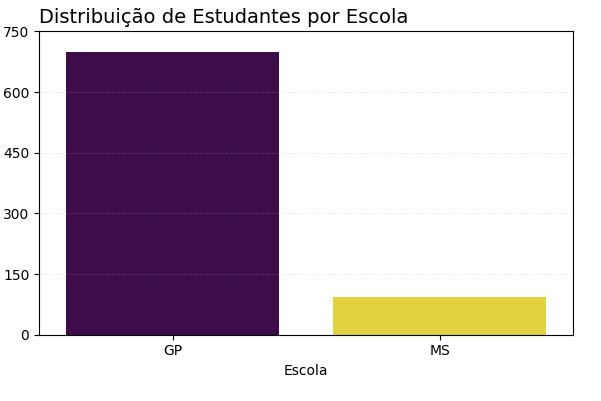
\includegraphics[keepaspectratio]{imagens/dist-estudantes.png}}

\subsection{Pontuação média os estudantes por
escola.}\label{pontuauxe7uxe3o-muxe9dia-os-estudantes-por-escola.}

\pandocbounded{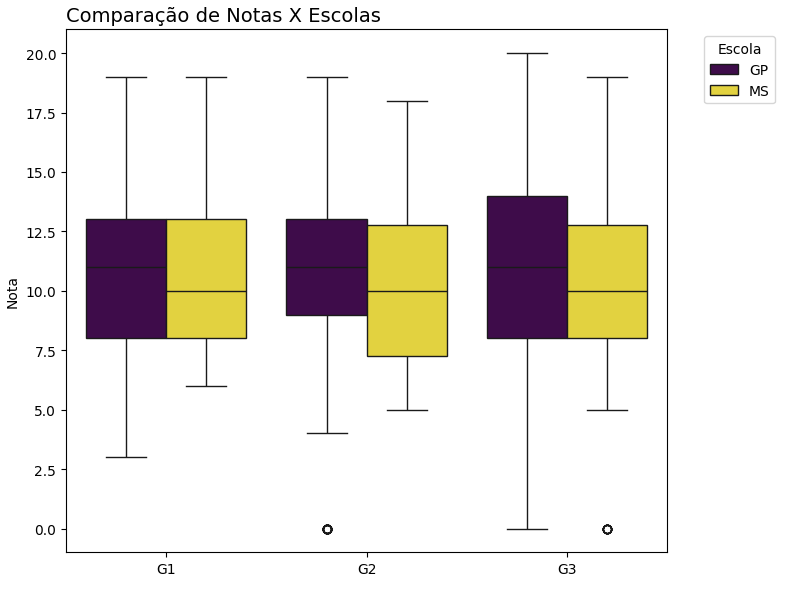
\includegraphics[keepaspectratio]{imagens/comp-notas-x-escolas.png}}

\subsection{Pontuação final média por faixa de faltas por
escola}\label{pontuauxe7uxe3o-final-muxe9dia-por-faixa-de-faltas-por-escola}

\pandocbounded{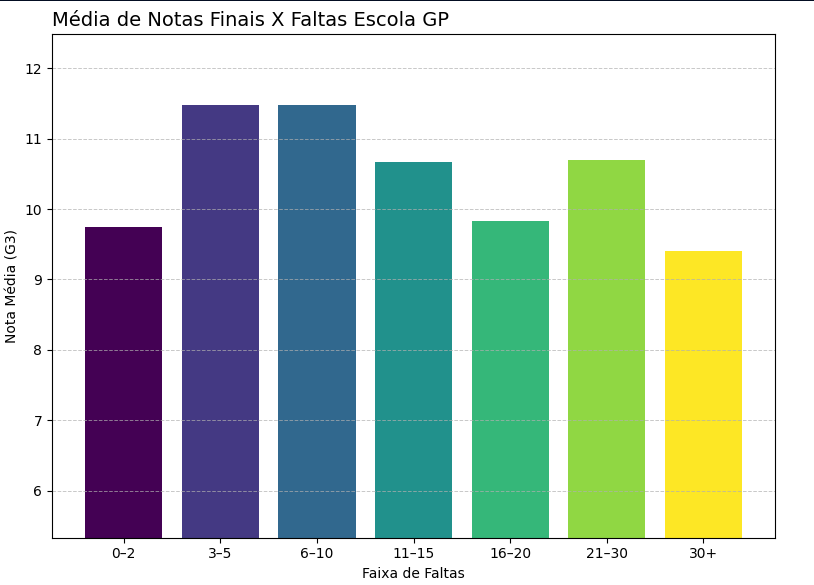
\includegraphics[keepaspectratio]{imagens/media-notas-GP.png}}
\pandocbounded{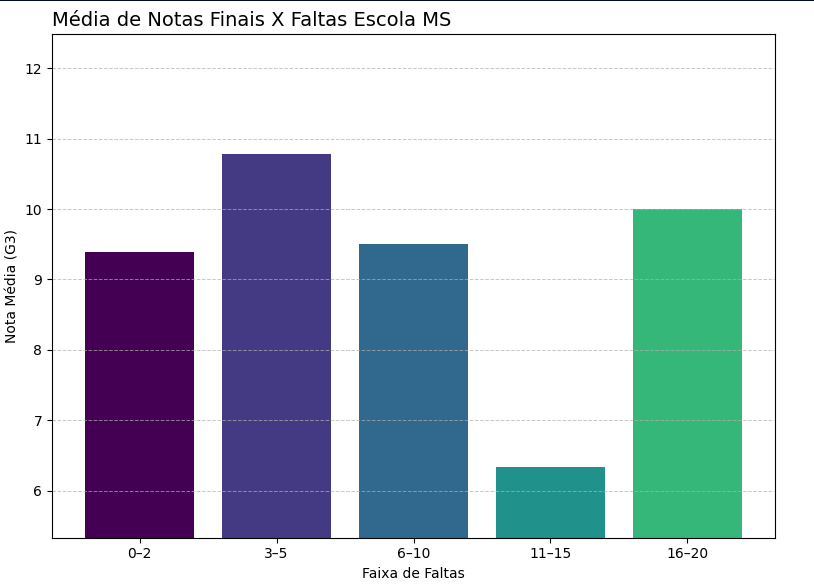
\includegraphics[keepaspectratio]{imagens/media-notas-MS.png}}

\subsection{A distribuição da frequência por
escola.}\label{a-distribuiuxe7uxe3o-da-frequuxeancia-por-escola.}

\pandocbounded{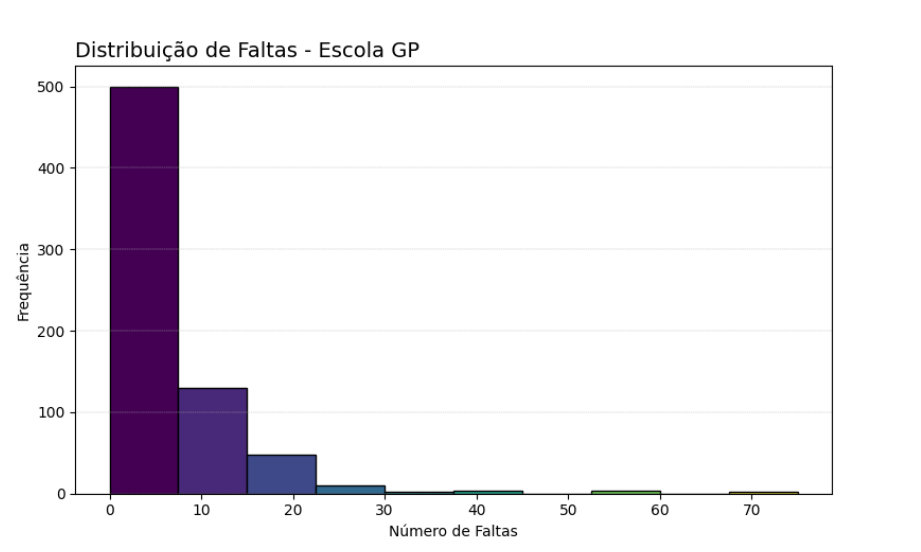
\includegraphics[keepaspectratio]{imagens/dist-faltas-E-GP.png}}
\pandocbounded{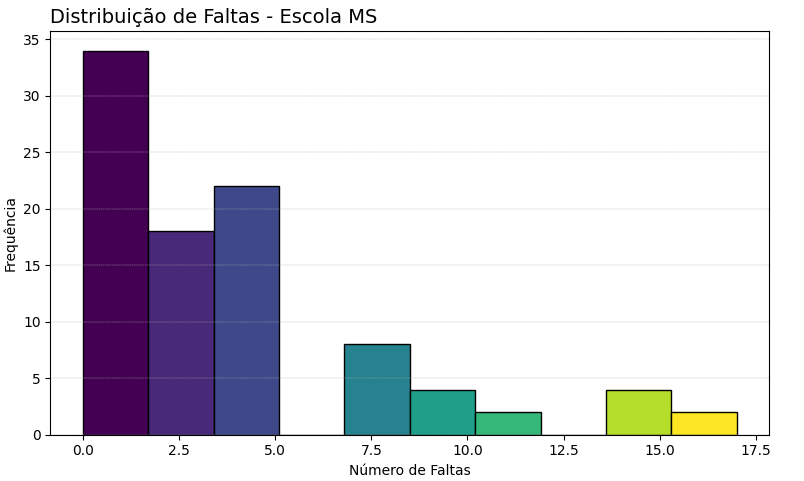
\includegraphics[keepaspectratio]{imagens/dist-faltas-E-MS.png}}

\subsection{Relação entre presença e
pontuação.}\label{relauxe7uxe3o-entre-presenuxe7a-e-pontuauxe7uxe3o.}

\pandocbounded{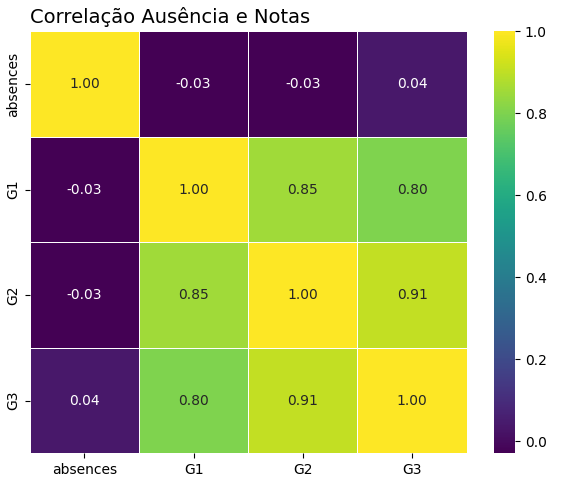
\includegraphics[keepaspectratio]{imagens/corr-aus-notas.png}}

\subsection{Correlação notas}\label{correlauxe7uxe3o-notas}

\pandocbounded{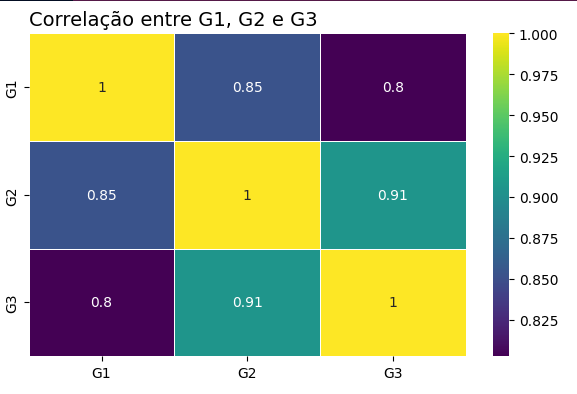
\includegraphics[keepaspectratio]{imagens/corr_notas.png}}

\subsection{Relação nota Parcial e
Final}\label{relauxe7uxe3o-nota-parcial-e-final}

\pandocbounded{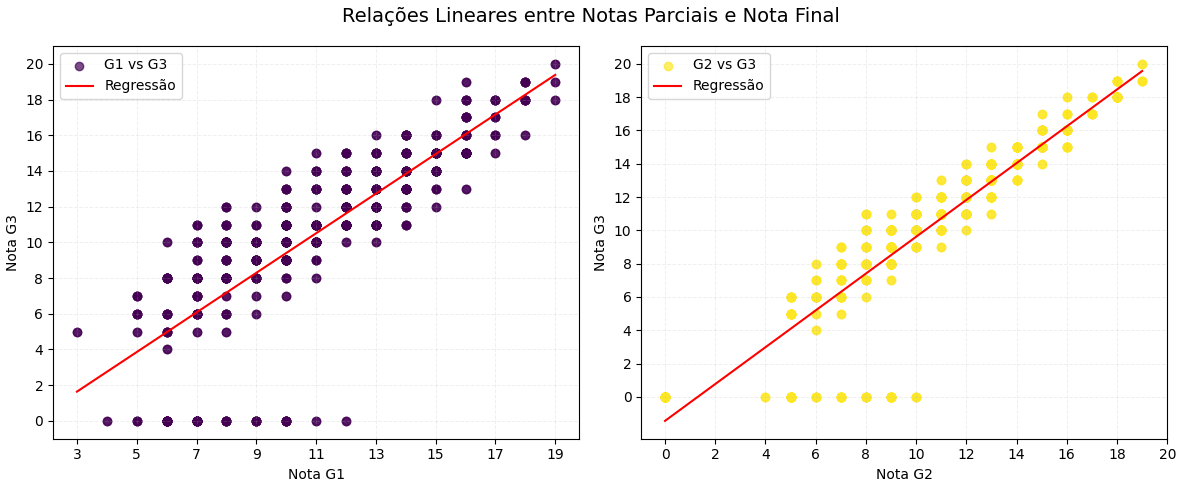
\includegraphics[keepaspectratio]{imagens/relacoes-lineares-notas.png}}

Essas avaliações evidenciaram uma tendência evidente: estudantes que
frequentam mais frequentemente tendem a alcançar melhores desempenhos
acadêmicos.

\section{Hiperparâmetros do Random Forest
Regressor:}\label{hiperparuxe2metros-do-random-forest-regressor}

\begin{itemize}
\item
  Quantidade de estimadores: 100
\item
  Profundidade máxima (max\_depth): Não definida (árvores se
  desenvolveram de forma autônoma)
\item
  Estado Aleatório: 42 (para replicabilidade)
\end{itemize}

\section{Dicionário de Dummys}\label{dicionuxe1rio-de-dummys}

\begin{longtable}[]{@{}
  >{\raggedright\arraybackslash}p{(\linewidth - 4\tabcolsep) * \real{0.2222}}
  >{\centering\arraybackslash}p{(\linewidth - 4\tabcolsep) * \real{0.0972}}
  >{\raggedright\arraybackslash}p{(\linewidth - 4\tabcolsep) * \real{0.6806}}@{}}
\toprule\noalign{}
\begin{minipage}[b]{\linewidth}\raggedright
Variável
\end{minipage} & \begin{minipage}[b]{\linewidth}\centering
Valor
\end{minipage} & \begin{minipage}[b]{\linewidth}\raggedright
Significado
\end{minipage} \\
\midrule\noalign{}
\endhead
\bottomrule\noalign{}
\endlastfoot
\textbf{schoolsup} & 1 & Aluno recebe suporte educacional extra \\
\textbf{famsup} & 1 & Aluno recebe suporte extra da família \\
\textbf{paid} & 1 & Aluno paga aulas extras \\
\textbf{activities} & 1 & Aluno participa de atividades
extracurriculares \\
\textbf{nursery} & 1 & Aluno frequentou o berçário \\
\textbf{higher} & 1 & Aluno pretende fazer curso superior \\
\textbf{internet} & 1 & Aluno tem acesso à internet em casa \\
\textbf{romantic} & 1 & Aluno está em um relacionamento romântico \\
\end{longtable}

\bookmarksetup{startatroot}

\chapter{Resultados}\label{resultados}

\section{Variaveis com Maior
Relevância:}\label{variaveis-com-maior-relevuxe2ncia}

\pandocbounded{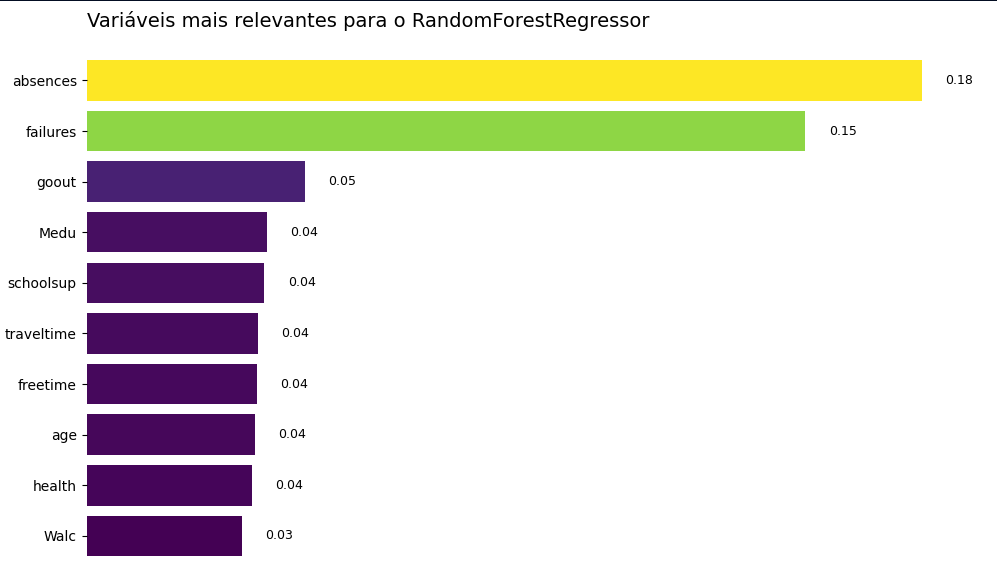
\includegraphics[keepaspectratio]{imagens/Relavancia-var.png}}

\textbf{Interpretação das variaveis: É notoória como para o modelo a
variavel} \(Absence\) (falatas/aussncia) se mostrou como a mais
relevante para a resolução do problema

\section{Métricas Random Forest
Regressor:}\label{muxe9tricas-random-forest-regressor}

\pandocbounded{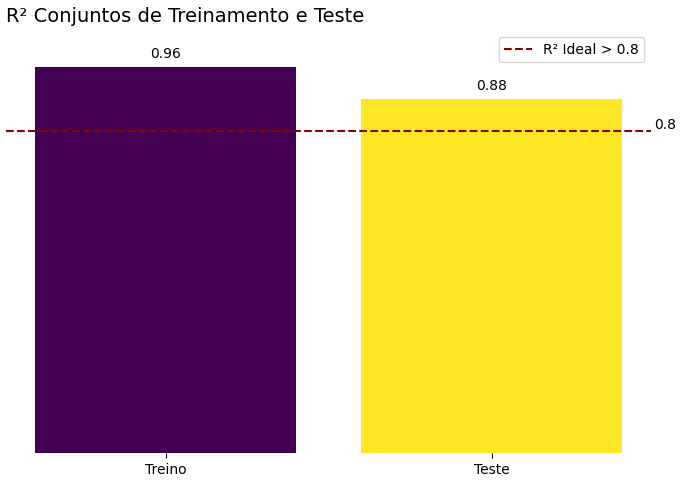
\includegraphics[keepaspectratio]{imagens/RFR-r2.png}}

Média R2: 0.82 Indica Bom ajuste; MAE: 1.25 Indica de baixa precisão
média; MSE: 2.79 Indica que o modedelo está dentro de uma faixa
tolerável, melhorando a precisão das previsões.

Esses achados corroboram a hipótese inicial: existe uma correlação
significativa entre a presença dos estudantes e suas notas.

Análise de Overfitting (RandomForest)

Observe se o R² de treinamento é similar ao de teste, indicando menor
propensão a overfiting

\section{Métricas Regressão liniear
:}\label{muxe9tricas-regressuxe3o-liniear}

\begin{itemize}
\tightlist
\item
  \textbf{Mean Absolute Error (MAE):} 3.41
\item
  \textbf{Mean Squared Error (MSE):} 20.27
\item
  \textbf{R-squared (R²):} 0.10
\end{itemize}

\section{\texorpdfstring{\textbf{Interpretação dos
modelos:}}{Interpretação dos modelos:}}\label{interpretauxe7uxe3o-dos-modelos}

Estratégias voltadas para o aumento da frequência dos alunos podem levar
a melhorias significativas no desempenho dos alunos. Essas percepções
foram cruciais para demonstrar aos interessados a viabilidade da
implementação do sistema RFID.

\bookmarksetup{startatroot}

\chapter{Conclusão}\label{conclusuxe3o}

Nossa análise mostrou que \textbf{faltar às aulas} \((Absence")\) é um
fator que mais pesa na previsão do desempenho dos alunos, com uma
importância de cerca de 0.18. Isso significa que quanto mais um aluno
falta, pior tende a ser seu desempenho. Nossos testes iniciais da
Regressão Linear também apontam para essa relação, mesmo que o resultado
do R² tenha dado 0.10 sugira que há mais a ser explorado.

Além disso, conseguimos criar um modelo preditivo usando Random Forest
que explica em média 82\% da variação nas notas dos alunos. Isso reforça
muito a ideia de que estar presente na escola é crucial para ir bem nos
estudos.

A tecnologia RFID surge como uma solução promissora para melhorar o
controle de presença, coletar dados automaticamente para análises
futuras e ajudar na administração da escola e os alunos. Com base nisso,
os próximos passos incluem criar um modelo experimental do sistema RFID
e coletar dados reais de presença com ele para deixar nosso modelo ainda
mais preciso.

É importante destacar que, apesar dessas descobertas claras, o
desempenho dos alunos é algo complexo e exige mais investigação. Por
isso, é fundamental expandir nossas análises para incluir outros
fatores, como a participação em atividades extras, o desempenho em
provas contínuas, o histórico escolar completo e, especialmente,
questões socioeconômicas dos alunos.

Em resumo, este projeto prova a importância do controle automático de
presença para o avanço acadêmico. Ele oferece uma base sólida para
futuras ações, mas também sublinha a necessidade de pesquisar mais a
fundo para entender todos os elementos que influenciam o sucesso
educacional.

Em resumo, com o RFID avançaremos na análise de dados por que
passaríamos a capitar algo algo que uma chamada normal não apresenta:\\

1 - Se o aluno aproveita o tempo todo de cada aula do ano ou não
(deixamos de ficar limitados a condição `binária' de Presença ou Falta;

2 - E assim testar se os alunos, em geral, chegam pontualmente, no
contexto do ceub às 8h e saem as 10:50h, apresentam melhor rendimento do
que outros que têm o costume de chegar atrasado (e o nivel de atraso),
ou quem têm o costume de sair bem mais cedo.

\bookmarksetup{startatroot}

\chapter{Referências}\label{referuxeancias}

As referências estão organizadas no arquivo \texttt{.bib} e serão
exibidas automaticamente.

\section{Base de dados utilizada}\label{base-de-dados-utilizada}

https://www.kaggle.com/datasets/whenamancodes/student-performance/data

\section{Estudo para o trabalho}\label{estudo-para-o-trabalho}

https://consortium.uchicago.edu/sites/default/files/2018-10/07\%20What\%20Matters\%20Final.pdf

\phantomsection\label{refs}




\end{document}
